\RequirePackage{filecontents}
\begin{filecontents}{\sample.bib}

\end{filecontents}
\documentclass{article}

% Language setting
% Replace `english' with e.g. `spanish' to change the document language
\usepackage[english]{babel}

% Set page size and margins
% Replace `letterpaper' with`a4paper' for UK/EU standard size

% Useful packages
\usepackage{amsmath}
\usepackage{graphicx}
\usepackage[colorlinks=true, allcolors=blue]{hyperref}


\begin{titlepage}
    \begin{center}
    
    \line(1,0){350}\\
    [0.5cm]
    \huge{\bfseries Stock Data Forecasting Using Deep Learning with Backtesting Strategies
}\\
    [1mm]
    \line(1,0){350}\\
    [2cm]
    \end{center}

    \par\medskip
    \begin{center}
    \hfill
    \begin{tabular}[t]{@{}l@{\hspace{5pt}}p{.17\textwidth}@{}}
    \textit{\underline{Submitted by:}}\\
    [0.5cm]
    Kamalhasan B   & a.narexxxxx@gmail.com\\
    Narendra A      &   kamxxxx@gmail.com\\
    \end{tabular}%
    \end{center}
    \end{titlepage}

\date{}

\begin{document}

\section{Introduction and Project background}

Stock data is a time series-driven data widely used in financial market analysis to identify market trends for better investments. Accurate forecasting of market trends plays a prominent role in this field of study. Since beginner traders are more likely than experienced traders to make mistakes and suffer heavy losses in the market, stock market prediction provides additional benefits for them. This project includes data acquisition, exploratory data analysis, data visualization, model development, and training, interpreting prediction results which are essential phases in the data life cycle.


\section{Problem Statement}
Fluctuations in stock prices affect investor perception and thus there is need for prediction of future prices. Market volatility depends on several factors that impact the price due to stocks' relative stability and predictability. Macro factors, regional factors, company, and market factors. Because of the non-linearity of the data, it is a challenging task for accurate forecasting using traditional machine learning techniques. We propose a deep learning model LSTM (Long short-term memory network) to discover future market trends by training the models with historical data.


\section{Related works}

In the research\cite{technical_indicators_forecasting}, the author concentrated on historical stock prices and used technical indicators to increase forecasting accuracy. This study's objectives are to gauge forecast precision and assess outcomes. Technical indications were employed as features in the prediction model, which was built using historical data. Utilizing extended short-term memory networks, the studies were carried out. Backtesting was carried out to demonstrate the final model's applicability in practical settings and gauge the profitability of the outcomes. The end results demonstrate that while it is not possible to anticipate a stock's exact price in the future in order to achieve profitable results, the author in the paper\cite{technical_indicators_forecasting} proposed that deep learning may be used to forecast stock market trends and produce buy and sell signals.

In the research\cite{forecasting_dl}The idea put out in this paper is that historical value, which may be utilized to forecast future movement, is what impacts all other market events. Using machine learning techniques, it is possible to identify paradigms and insights that can be applied to create unexpectedly accurate predictions. The Long Short Term Memory model is suggested using to look at a stock's potential future price. In order to make better, more knowledgeable investing decisions, this study will attempt to forecast stock market values. Finally, the author in this research proposed LSTM model with more inputs might further improve this by extracting pertinent data by using additional input gates with low correlated variables to eliminate their noise influenced by mainstream factors. Several other methods have been tested using a combination of machine learning and deep learning techniques\cite{forecast_DL_ML} and \cite{forecast_ML} which concluded more research can be done on LSTM models suitable for stocks price forecasting.

\section{Objective}

The objective of this study is to forecast the future stock prices of companies listed in the S&P500 by identifying the trends in the historical data. The chosen companies list is Google, Apple, Cisco, Dominos.

\section{Data Collection}

The dataset is extracted from yahoo finance API. Dataset consists of Date, Open price, High price, low price, closing price, and volume information for companies Apple(AAPL), Google(GOOG), Cisco(CSCO), and Domino's(DPZ). Data is extracted between 2011-01-01 till 2021-12.30 a total of 11 years. Each stock's price information contains data from 2011 to 2021 on a daily interval, which makes more than 2768 records for each company. The code extracts the dataset through this API during run time to evaluate and execute the results. A sample snippet of data extracted is shown in the below figure.

\begin{center}
    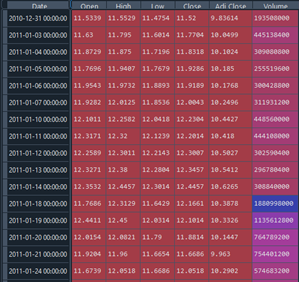
\includegraphics[width=11cm]{data_extraction.png}
    \caption{ Figure representing sample data extracted}
\end{center}

\section{Exploratory Data Analysis}

A suitable method for comprehending and evaluating the data sets is exploratory data analysis. Data scientists and analysts frequently utilize this technique to highlight key aspects of data sets and display them using various graphs and charts. It aids data scientists in their efforts to find patterns, identify anomalies, or validate presumptions. Here we have generated graphs related to closing prices, the volume of the stocks sold, daily returns, and the correlation between the data points.

\begin{center}
    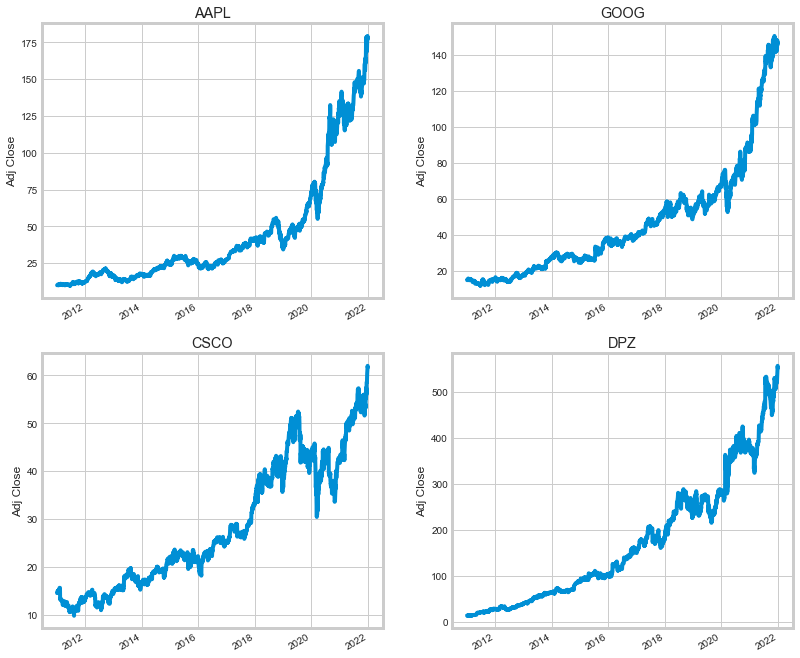
\includegraphics[scale=0.40]{close_prices.png}
    \caption{ Above figure indicating the closing prices of individual stocks}
\end{center}

\begin{center}
    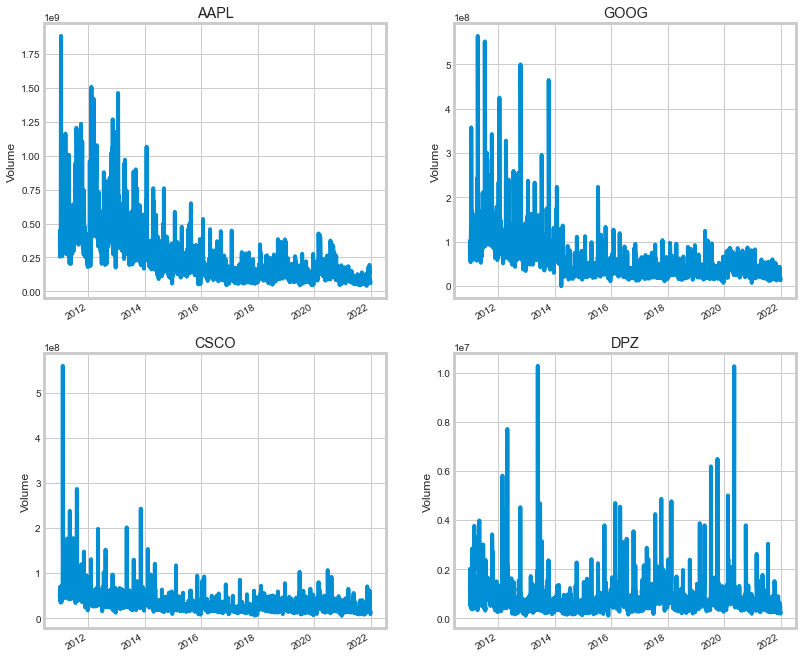
\includegraphics[scale=0.40]{volume_info.png}
    \caption{ Above figure indicating the volume of individual stocks}
\end{center}

\begin{center}
    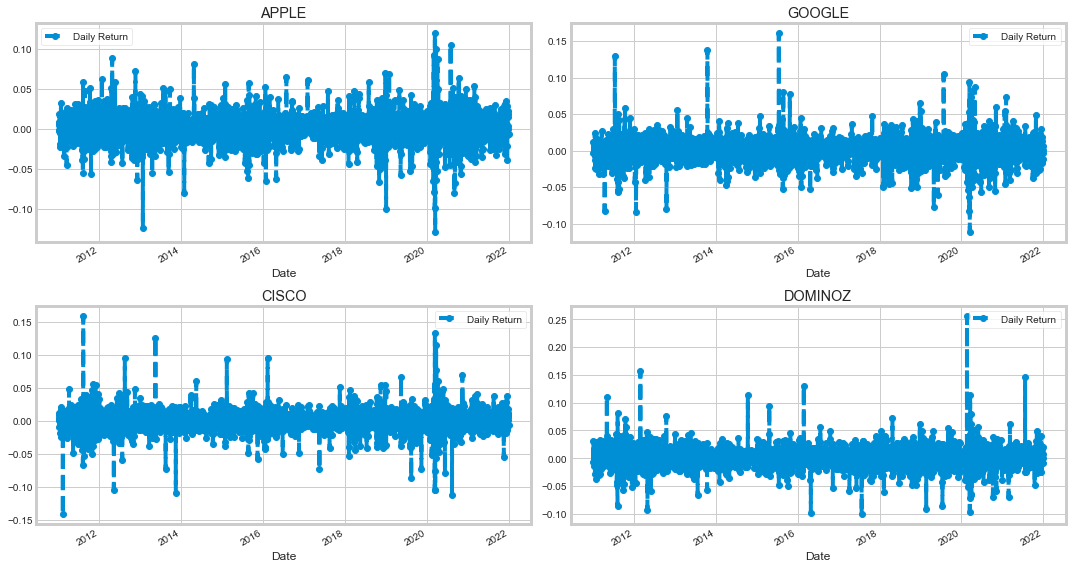
\includegraphics[scale=0.40]{daily_returns.png}
    \caption{ Figure indicating the daily returns calculated based on the present and previous day}
\end{center}

\begin{center}
    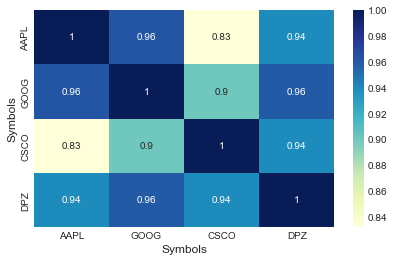
\includegraphics[scale=0.80]{heatmap.png}
    \caption{ Figure representing the correlation of closing prices between company stocks chosen}
\end{center}
\newpage
From the above correlation matrix, it can be observed that the individual closing price of the company is correlated to other closing prices. So, a single model developed can efficiently work on all the company closing prices forecasting from the chosen list.

\begin{center}
    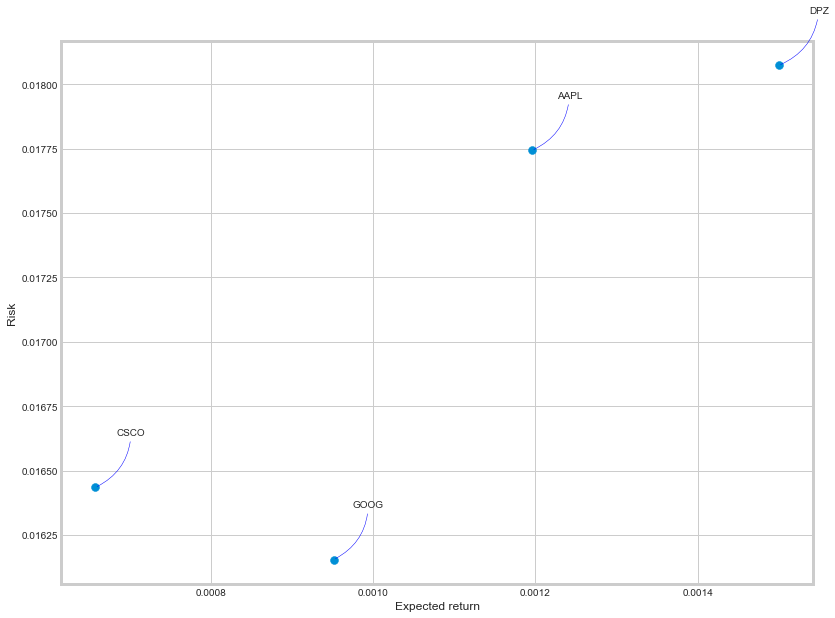
\includegraphics[scale=0.40]{risk_plot.png}
    \caption{ Figure representing risk information based on the expected returns}
\end{center}

\section{Design and Methodology}

Data extraction through the yahoo API endpoint is the first stage of this project, followed by data collection. Open, high, low, close, and volume information of the selected list of companies are included. The future close price is predicted by this approach using a close price. EDA tasks like locating correlations and identifying and imputing missing data points are carried out using the extracted data. Further, LSTM model is used to estimate future prices by training it on historical data. Developed model is trained on a batch size of 30 for 50 epochs in total to reduce the loss. By including one more layer and altering the activation, hyperparameter tuning is carried out at this step. To improve forecasting results, this hyperparameter needs to be modified during model training. The moving average back testing technique will then be applied to the anticipated results.

\begin{center}
    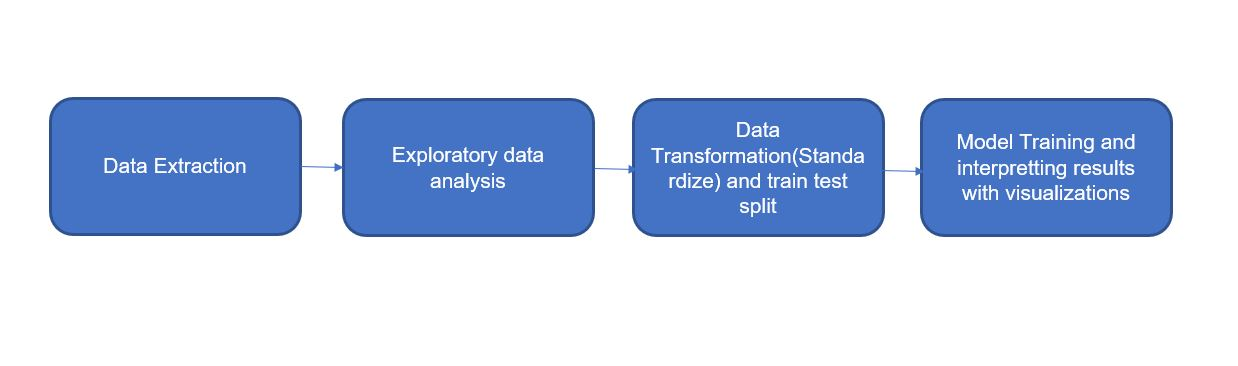
\includegraphics[width=\textwidth]{methodology.JPG}
    \caption{Blueprint representing the research design}
\end{center}


\section{Conceptual Framework}
Different data processing and data transformation techniques have been employed in developing this project. After the data extraction is done, we filter the data for the closing price as it is the variable that is been focusing on forecasting. As our data points differ greatly between the range, an initially standard scalar is applied to the data to perform the transformation to a range between 0 to 1. In this process, MinMaxScaler function is used from scikit-learn for transformation. Further the data is splitted at 70 and 30 percent for training and testing using train test split function from the scikit-learn module.

Our model makes predictions as well as random biases and weights by feeding data to the present neural network, which is a component of model training. The LSTM model developed contains nine levels, including the input layer, four LSTM layers (hidden layers), four dropout layers, and an output layer with the activation function tanh. Each unit in a layer connects to all units in neighboring layers. The output layer, which has one thick layer unit, creates the fully connected layer. As a part of hyperparameter tuning activation function of the layers is changed to 'relu' based on the information provided by author in \cite{forecasting_dl}. Several other parameter tuning is performed by adding one extra LSTM layer to the network, but the network lags far behind in this case. 
Architecture of the LSTM model developed is shown below image.

\begin{center}
    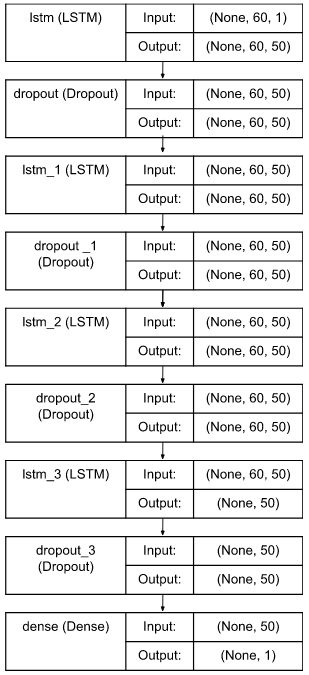
\includegraphics[scale=0.70]{model_summary_01.png}
    \newline
    \caption{LSTM model summary representing layers}
\end{center}

\section{Implications of Study}
Stock data forecasting depends on various factors. In the present day, social media posts are also playing a prominent role in the volatility of the market. In the research, \cite{implications} author has mentioned how stock prices are affected by news sentiments. Natural language processing-based sentiment analysis is chosen by the author to get the feeds from social media channels through a dictionary-based sentiment analysis model. Historical data is useful in learning the patterns but this method should be included to accurately predict future prices which takes a long research work.


\section{Data Visualization ad Results}

During the model training, the losses of the model were captured and plotted respectively. During the model training, a validation set is not provided to the data. 30 percent of the data is used for testing the model performance. In this section, the losses and the prediction results are visualized and discussed.

\begin{center}
    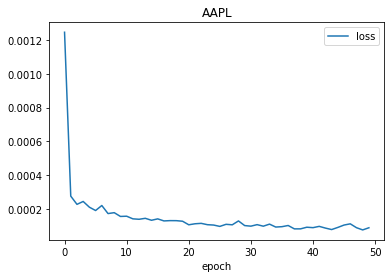
\includegraphics[scale=0.50]{loss_AAPL.png}
    \newline
    \caption{Training loss for Apple}
\end{center}

\begin{center}
    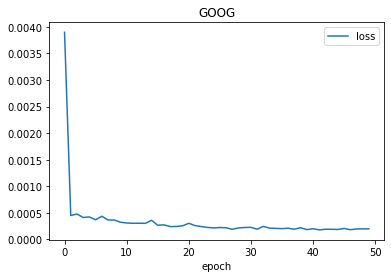
\includegraphics[scale=0.50]{loss_GOOG.png}
    \newline
    \caption{Training loss for Google}
\end{center}

\begin{center}
    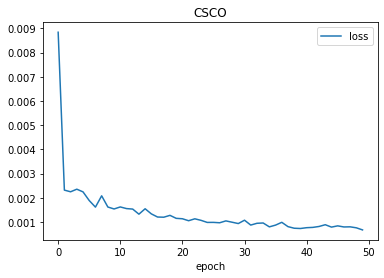
\includegraphics[scale=0.50]{loss_CSCO.png}
    \newline
    \caption{Training loss for Cisco}
\end{center}

\begin{center}
    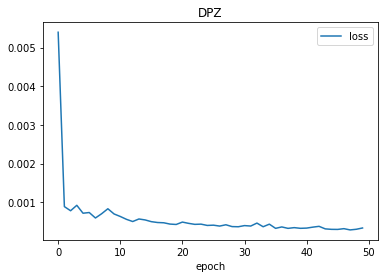
\includegraphics[scale=0.50]{loss_DPZ.png}
    \newline
    \caption{Training loss for Domino}
\end{center}

Below are figures representing the test data representing and prediction data from our trained models comparatively. We can observe the results from the model containing 5 LSTM layers and relu activation function are more diverged and resulted in greater root mean square error values.

\begin{center}
    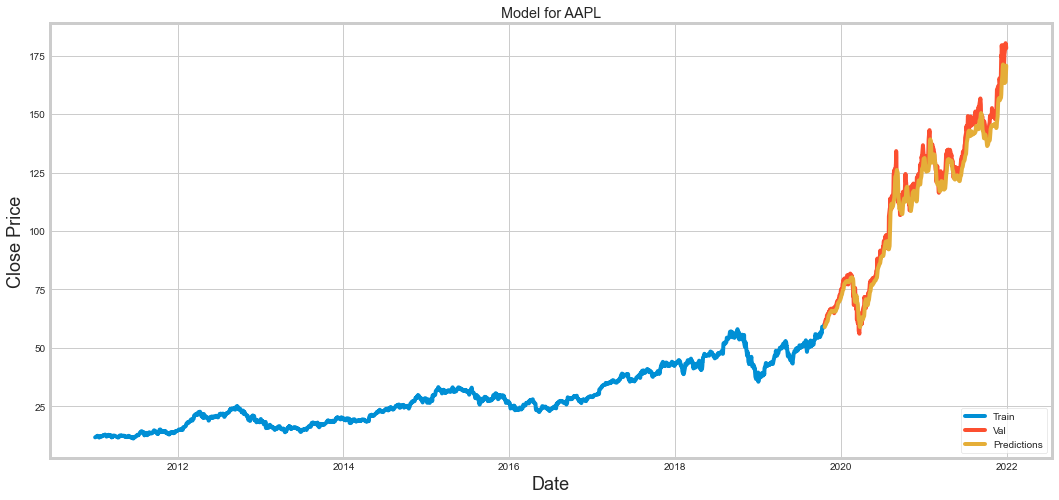
\includegraphics[width=\textwidth]{AAPL_results_01.png}
    \caption{Model with tanh as activation function and 4 LSTM layers(RMSE = 5.037)}
\end{center}

\begin{center}
    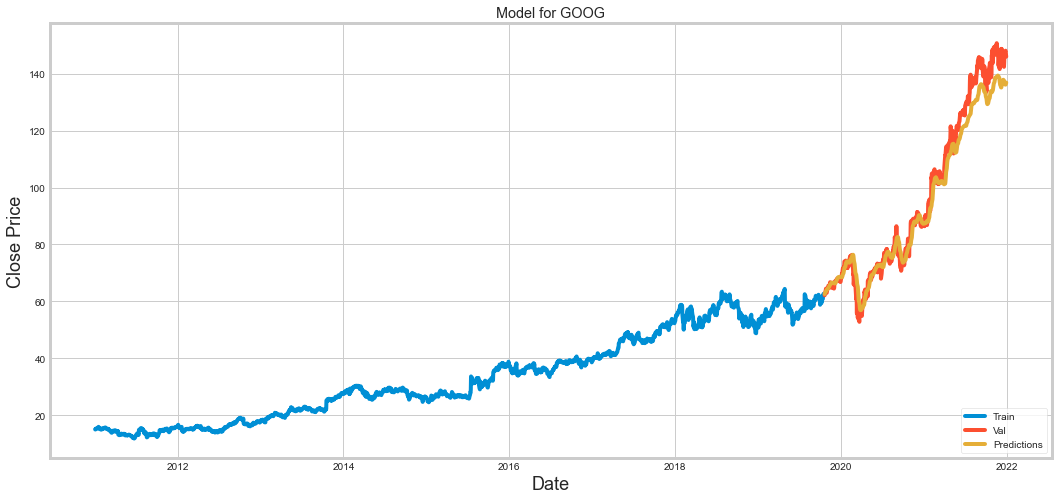
\includegraphics[width=\textwidth]{google_results_01.png}
    \caption{Model with tanh as activation function and 4 LSTM layers(RMSE = 5.269)}
\end{center}

\begin{center}
    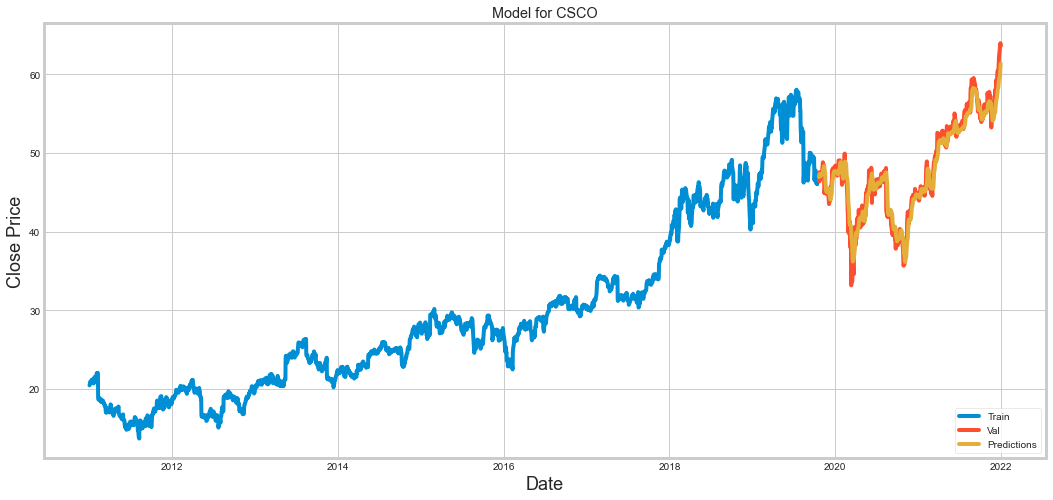
\includegraphics[width=\textwidth]{csco_results_01.png}
    \caption{Model with tanh as activation function and 4 LSTM layers(RMSE = 1.299)}
\end{center}

\begin{center}
    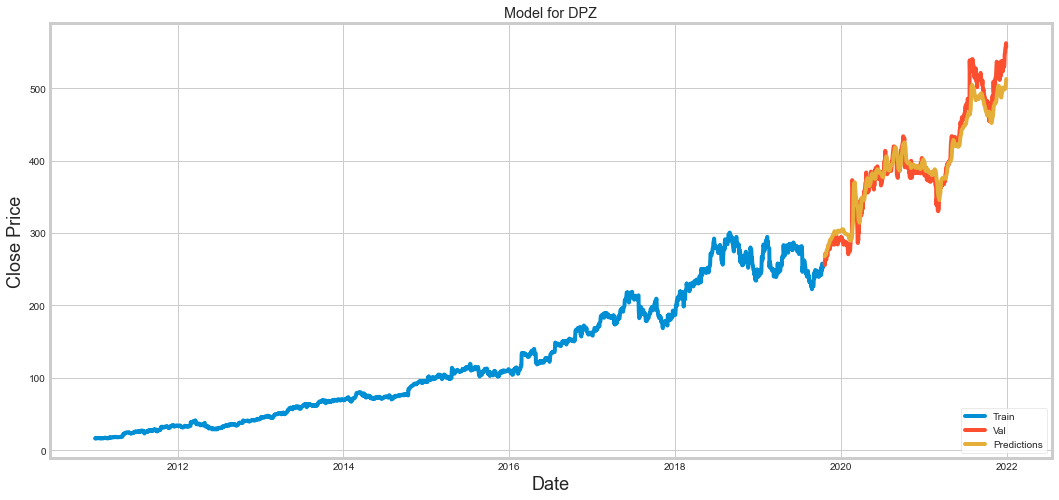
\includegraphics[width=\textwidth]{DPZ_results_01.png}
    \caption{Model with tanh as activation function and 4 LSTM layers(RMSE = 18.291)}
\end{center}

\begin{center}
    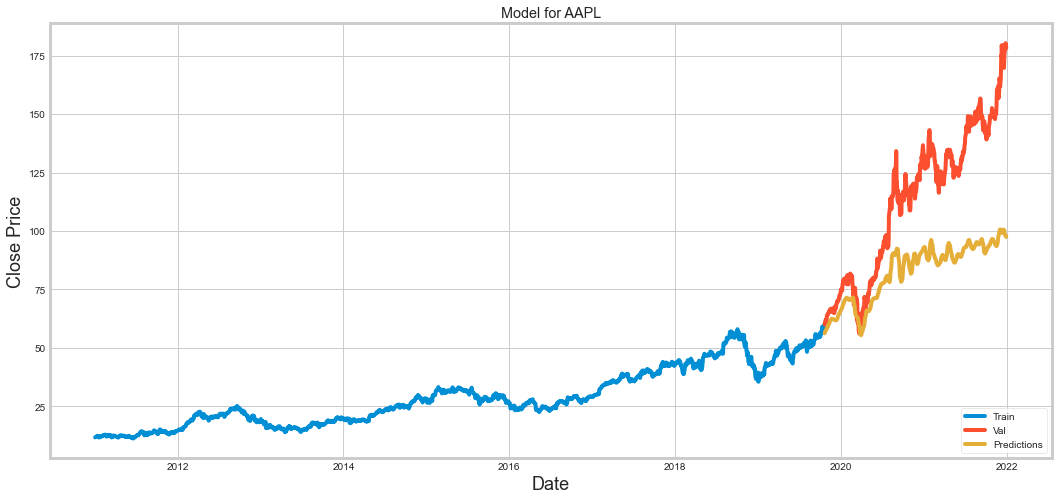
\includegraphics[width=\textwidth]{AAPL_results_02.png}
    \caption{Model with relu as activation function and 5 LSTM layers(RMSE=36.689)}
\end{center}

\begin{center}
    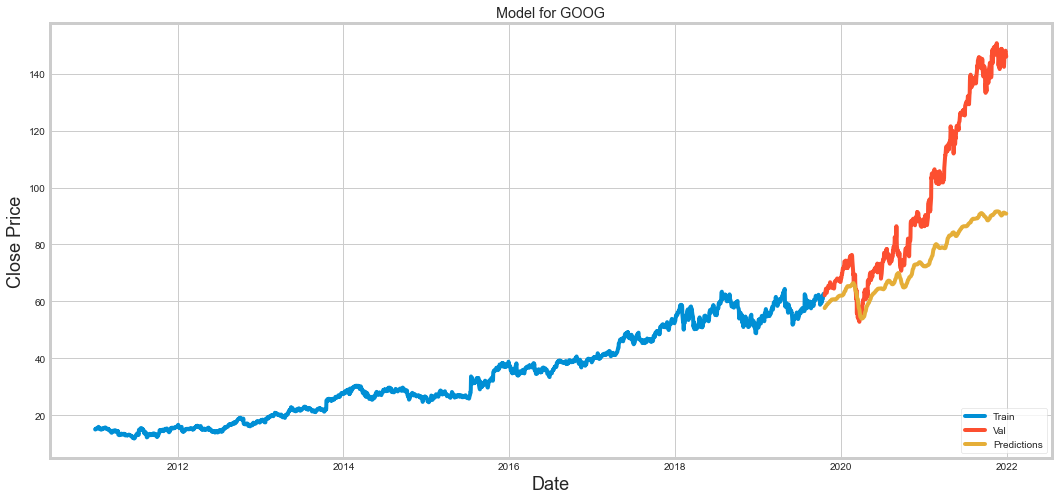
\includegraphics[width=\textwidth]{google_results_02.png}
    \caption{Model with relu as activation function and 5 LSTM layers(RMSE=29.439)}
\end{center}

\begin{center}
    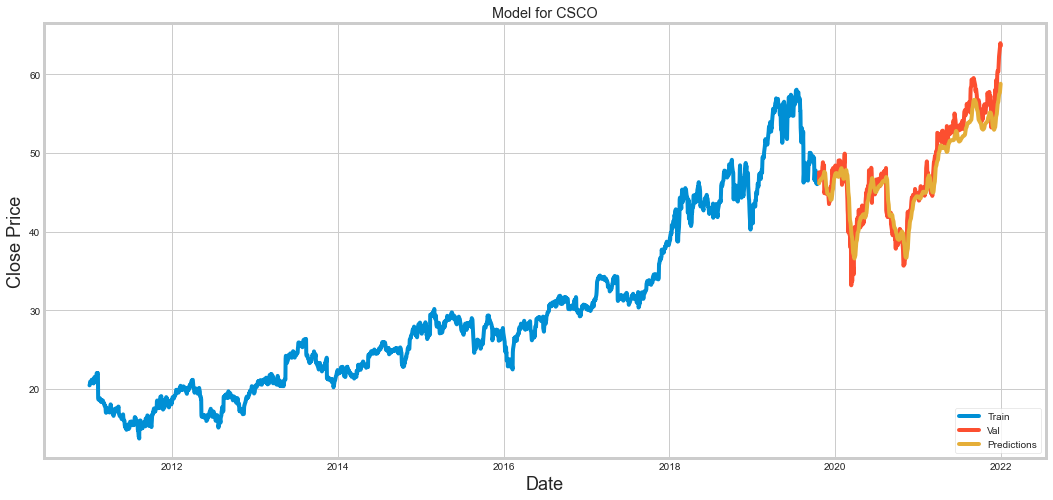
\includegraphics[width=\textwidth]{csco_results_02.png}
    \caption{Model with relu as activation function and 5 LSTM layers(RMSE=1.950)}
\end{center}

\begin{center}
    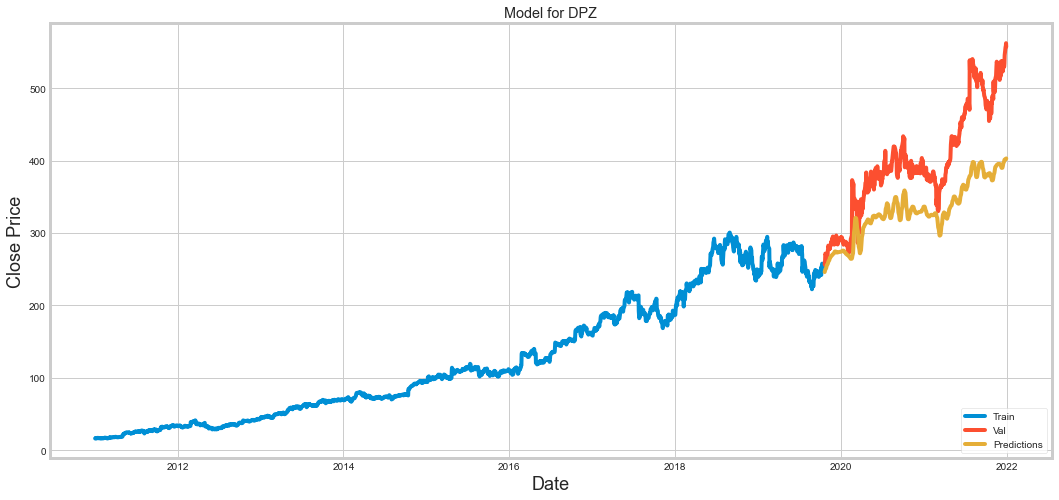
\includegraphics[width=\textwidth]{DPZ_results_02.png}
    \caption{Model with relu as activation function and 5 LSTM layers(RMSE=77.074)}
\end{center}

\begin{center}
    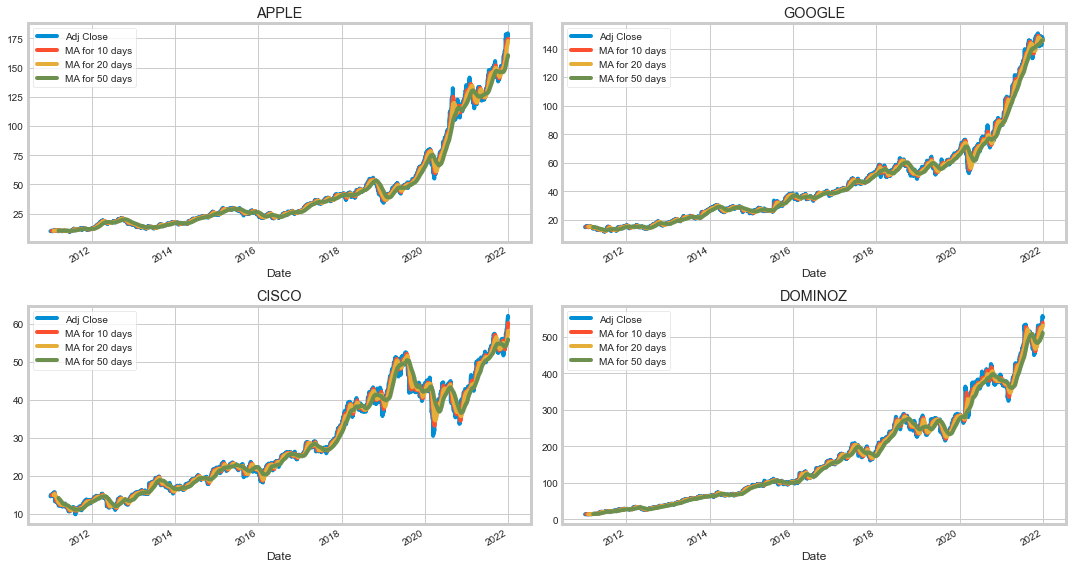
\includegraphics[width=\textwidth]{backtest_plot.png}
    \caption{Moving average calculated for duration of 10, 30, 60 days respectively}
\end{center}

From the above graphs we can clearly observe that the model with 5 layers and activation function lags behind our model built on 4 layers and tanh as activation function. The RMSE values represented below the figures show the predictions have more diverged from the actual. As a part of the qualitative analysis, the graphs in the moving average are less diverged and gives accurate predictions when compared to our forecasting results. Where as the model with 5 LSTM layers and relu activation is more diverged from the actual test data. So the model with four LSTM layers with tanh activation function is finally chosen.

\section{Conclusion}

In this project, a Long Short-term memory network to predict the closing prices of the stocks is developed by hyperparameter tuning on the activation function and changing the number of layers in the model. From the above results based on the root mean squared values and qualitative analysis from graphs, model performance is better for AAPL, GOOG, CSCO. Increasing the number of layers increased the forecasting errro rate. Further research can be done on investigating on LSTM model with a combination of machine learning models as a part of feature extraction process.

\bibliographystyle{plain}
\bibliography{sample}

\end{document}